\chapter{Резекційна хірургія печінки}

\section{Що таке резекція печінки?}

Резекція печінки -- хірургічна операція по видаленню ураженої частини печінки. 

\begin{figure}
  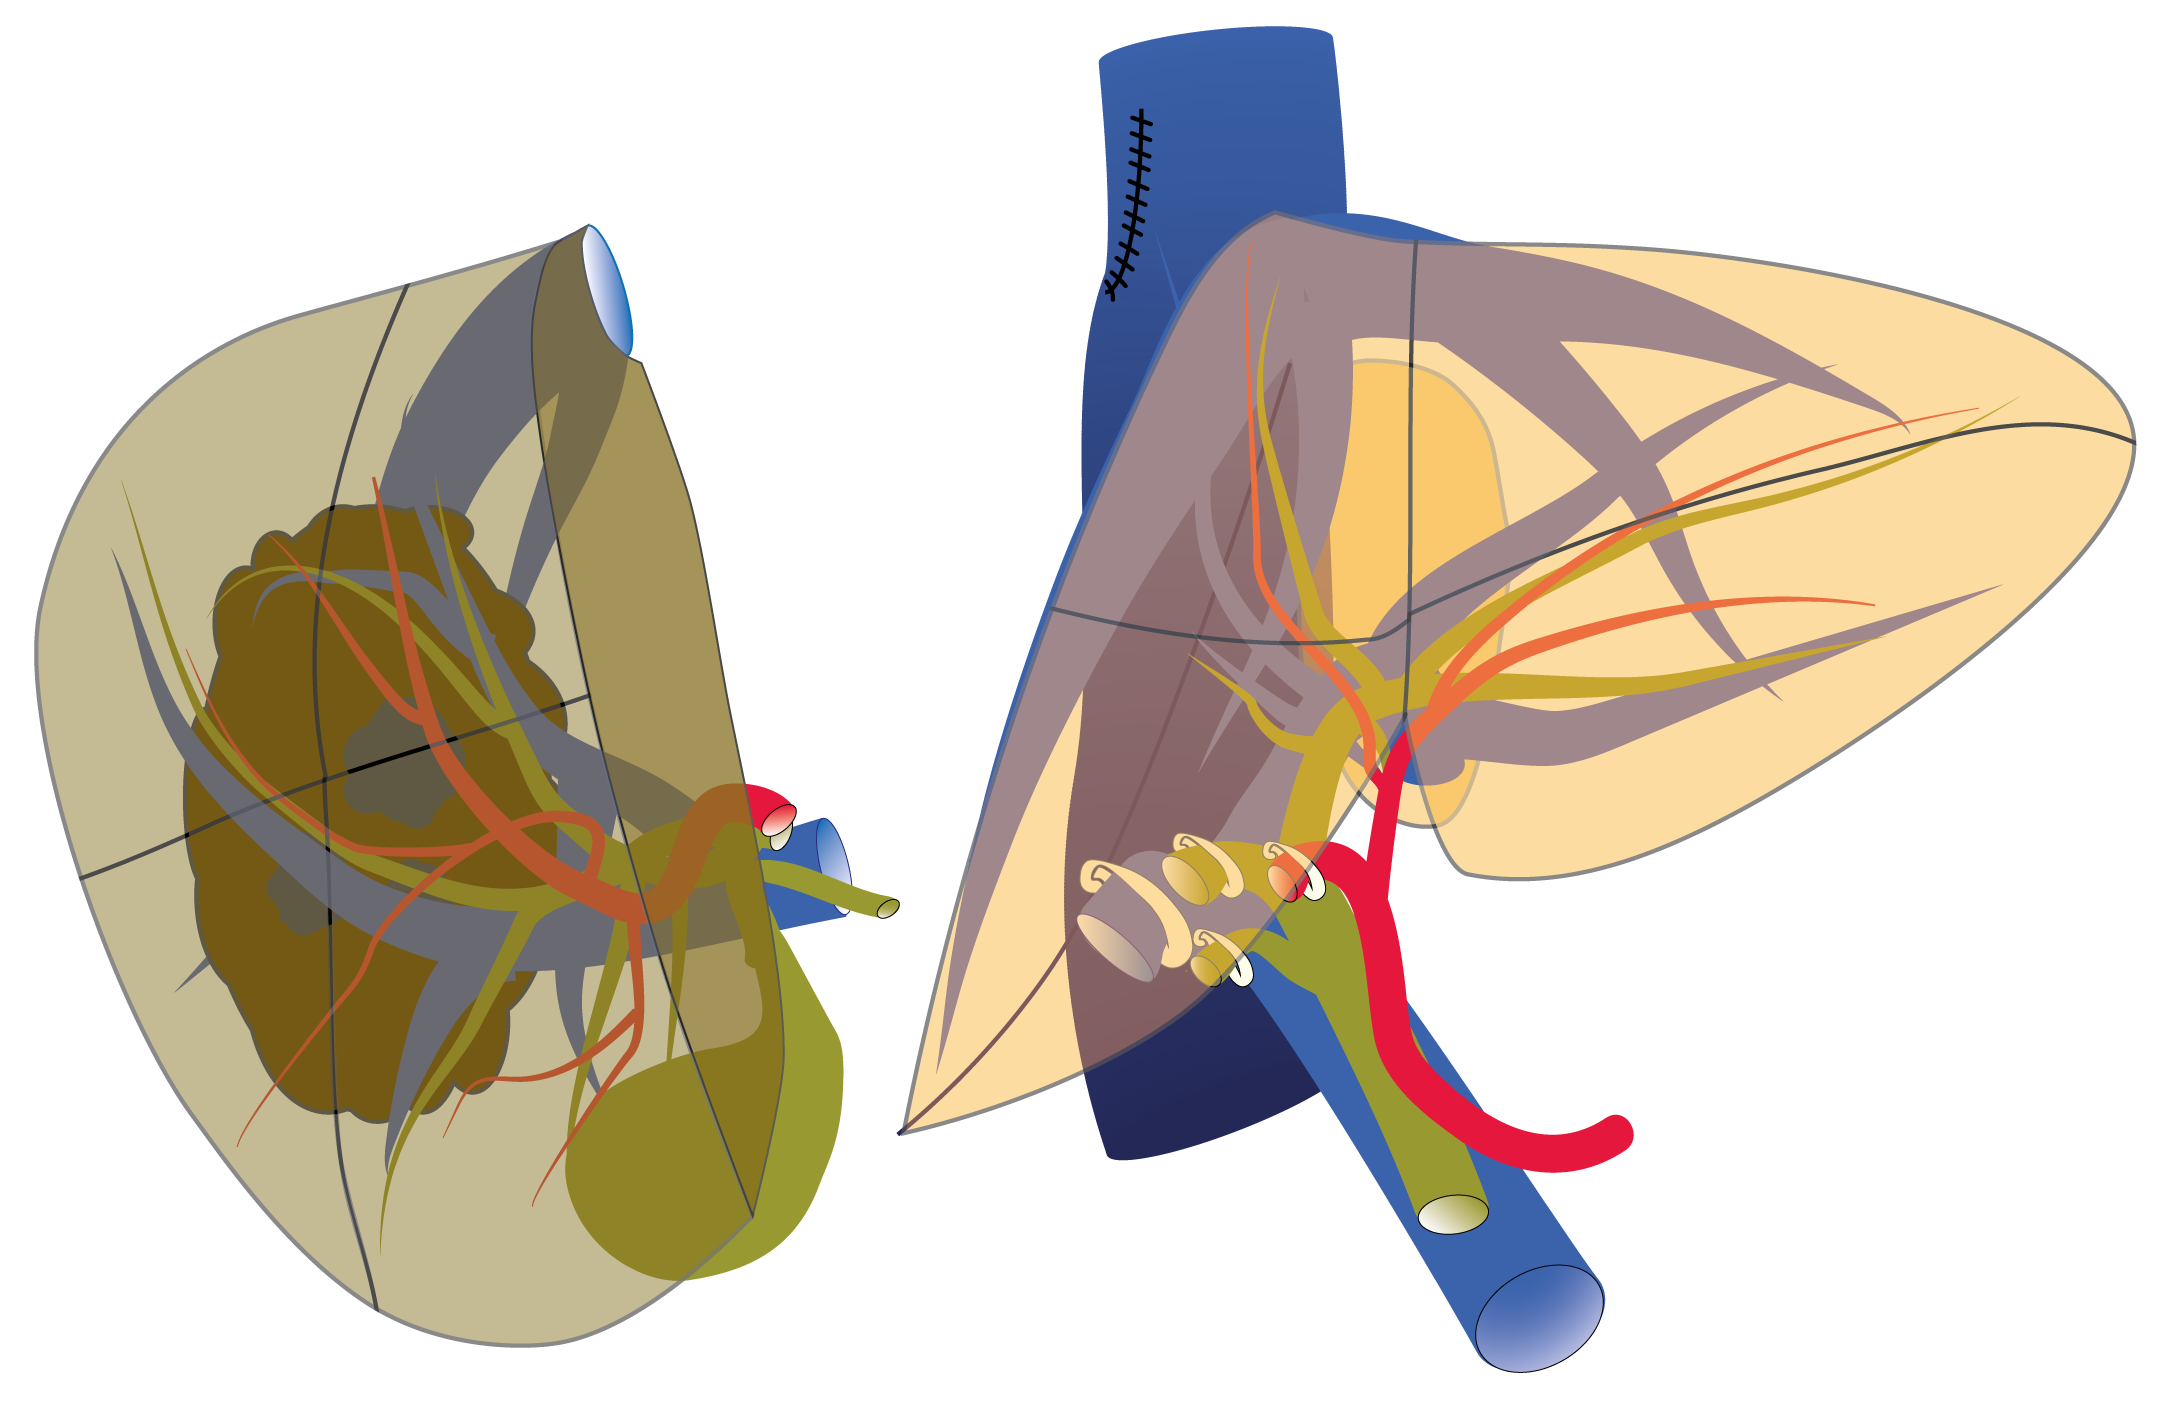
\includegraphics[width=\linewidth]{Figures/Right hepatectomy_Resection.png}
%  \checkparity This is an \pageparity\ page.%
  \caption{Резекція печінки - правобічна гемігепатектомія. Хірург виділяє та перев'язує всі судини, що живлять праву частку печінки, після чого видаляє паренхіму, що містить пухлину. Видалення жовчного міхура є одним з обов'язкових етапів цієї операції.}
  \label{fig:textfig}
  %\zsavepos{pos:textfig}
\end{figure}

Сучасні можливості гепатобіліарної хірургії дозволяють безпечно, із рівнем ускладненнь менше 10\%, виконувати резекцію печінки при ураженні пухлиною близько 70\% тканини печінки. 


\section{При яких захворюваннях необхідна резекція печінки?}

Резекція печінки є методом лікування вогнищевої патології печінки. ЇЇ виконують при злоякісних та доброякісних пухлинах печінки, кистах та хронічних абсцесах печінки.


\section{Які особливості резекцій печінки при онкологічній патології?}

Технічно резекції печінки при онкологічних пухлинах більш обширні та складні, так як можуть потребувати резекції та реконструкції судин чи жовчних протоків, лімфаденектомії та резекції суміжних органів при їх пухлинній інвазії. 

\begin{marginfigure}%
  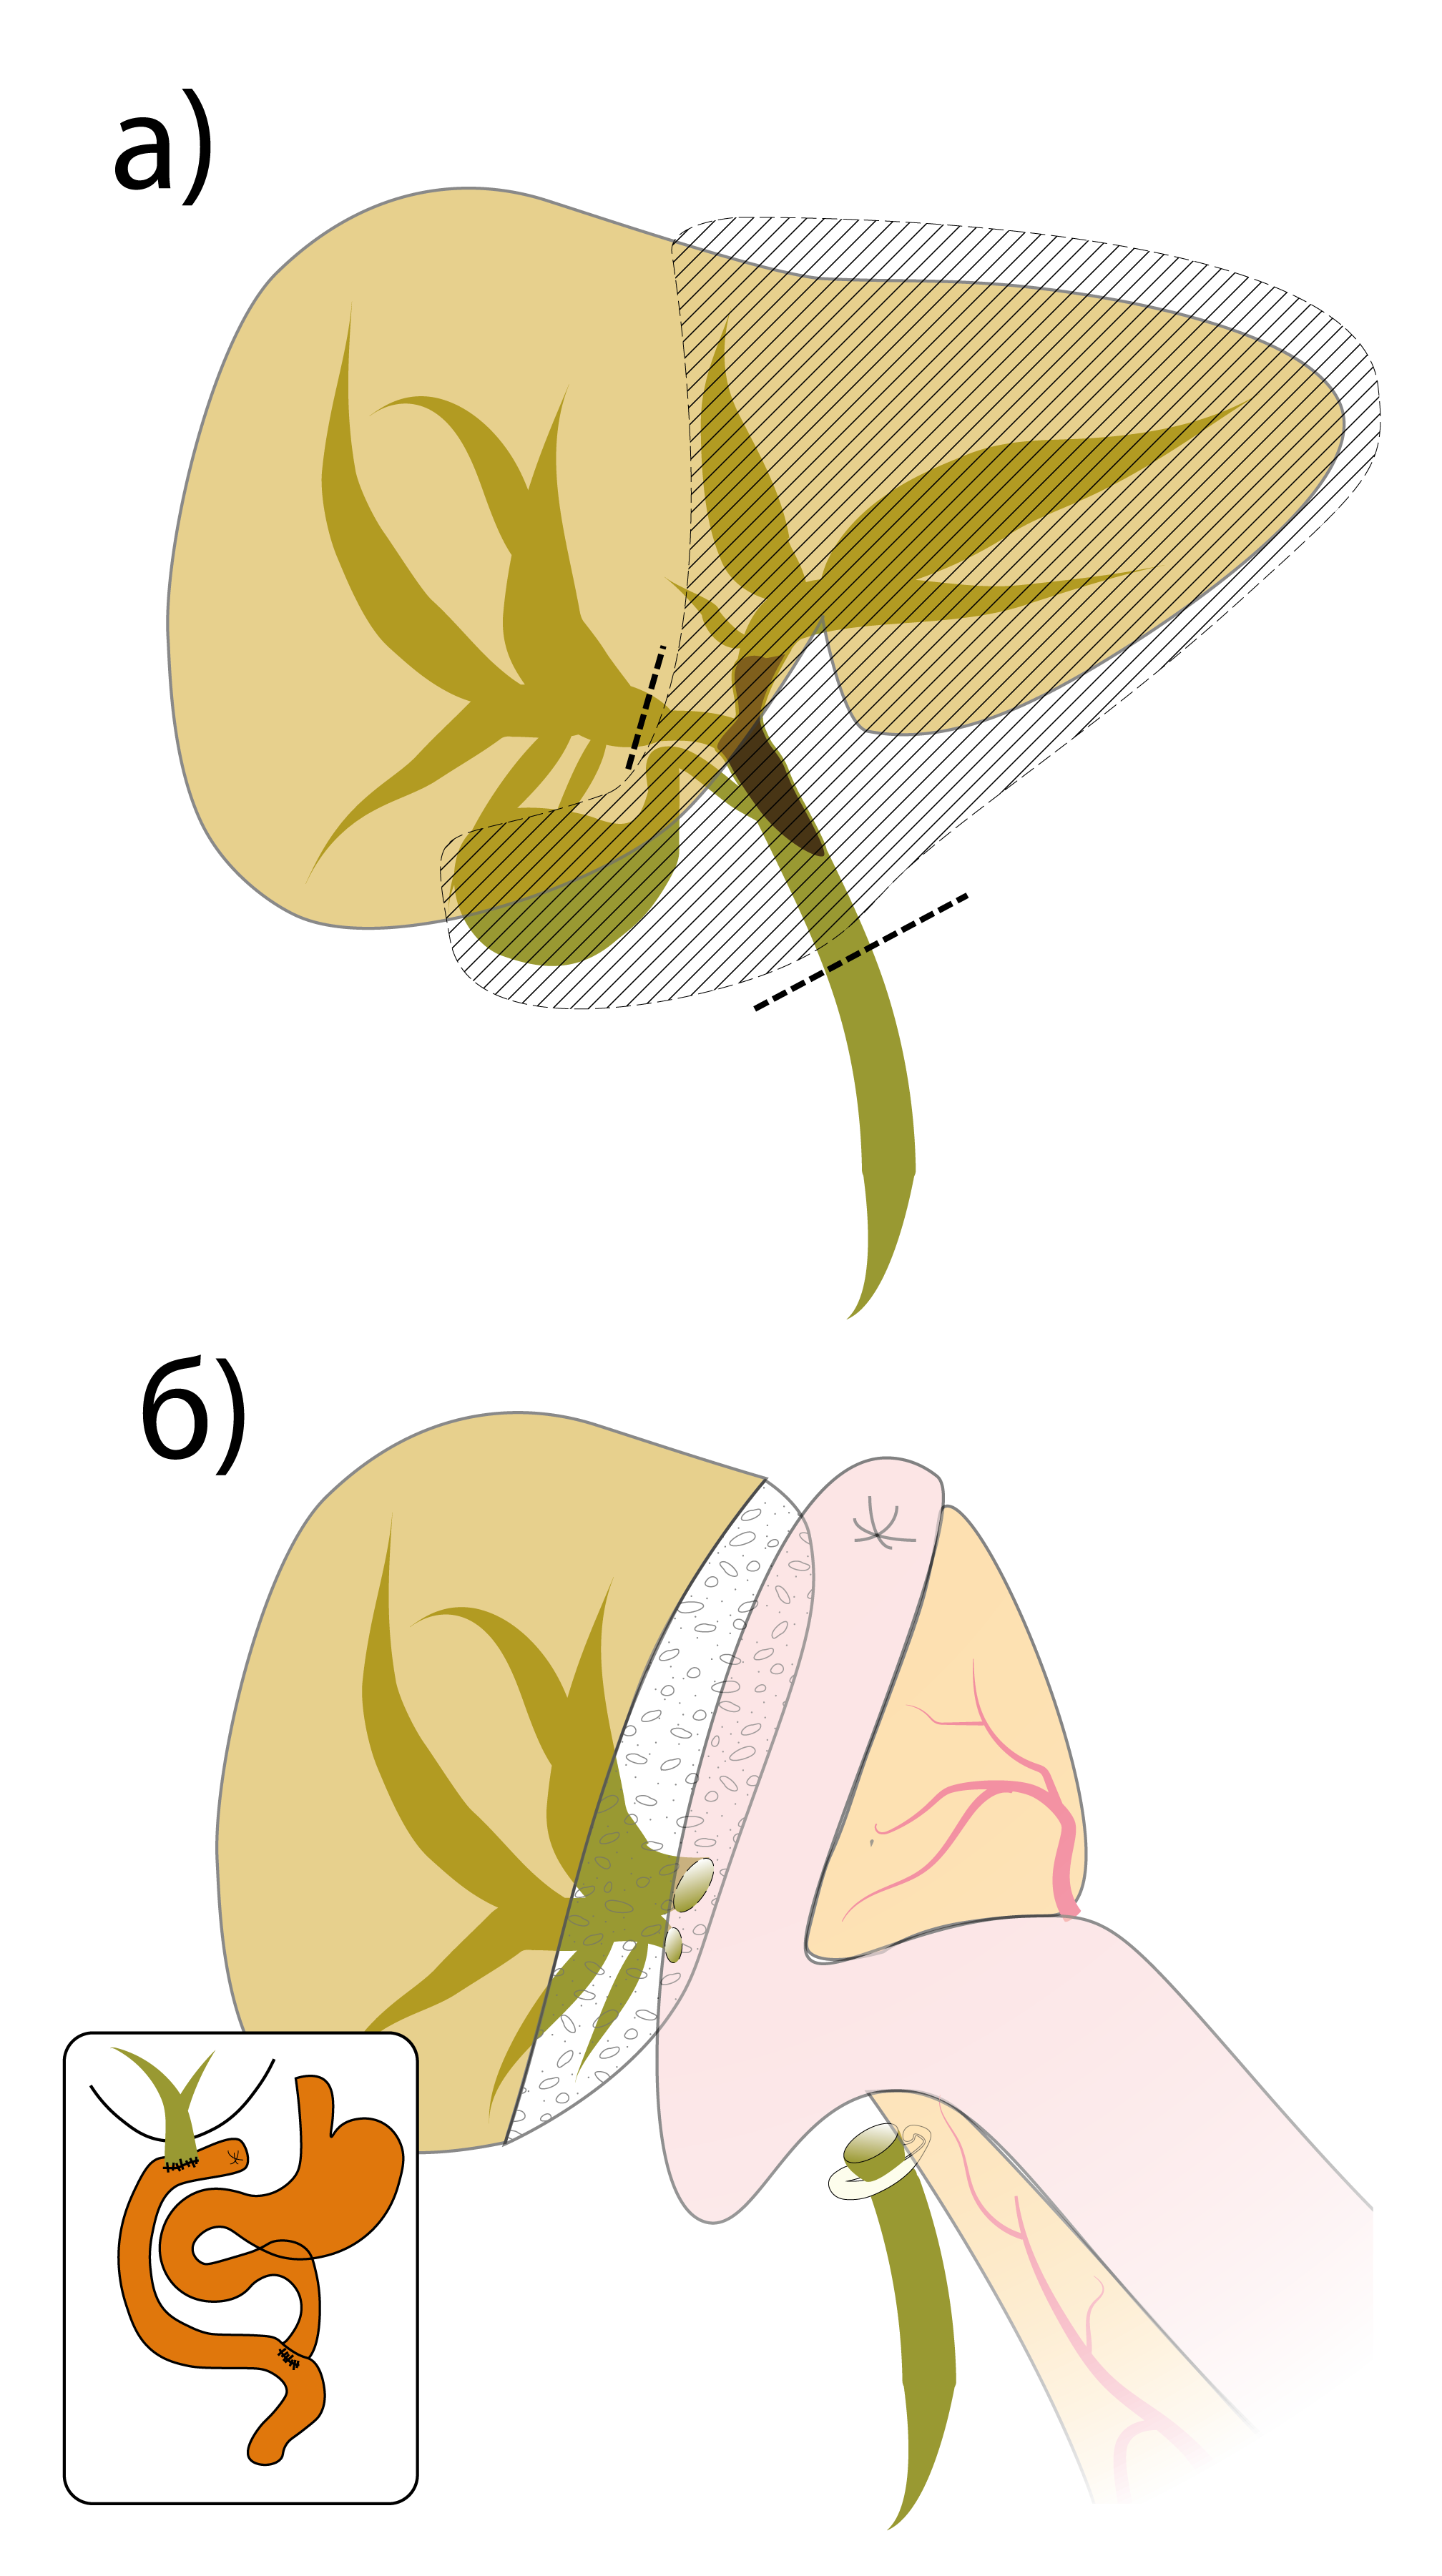
\includegraphics[width=\linewidth]{Figures/Bile duct resection.png}
  \caption{Резекція та реконструкція жовчних шляхів при пухлинному ураженні. 
  а) планований до видалення об'єм печінки (помічено сірою штриховкою), який включає печінку з пухлиною та уражені нею жовчні шляхи; б) реконструкція -- вільний від пухлини край жовчних шляхів зшивається із петлею тонкої кишки для відводу туди жовчі}
  \label{fig:crlm}
\end{marginfigure}

\begin{tcolorbox}[width=\textwidth,colback=red!5!white,colframe=red!75!black]    
Онкологічні захворювання -- складна проблема, яка потребує мультидисциплінарного підходу. Резекція печінки є формою локального контролю пухлини, що  застосовується в комбінації із іншими способами лікування. 
\end{tcolorbox}    


Необхідність проведення додаткового лікування перед чи після резекції печінки (наприклад адьювантної хіміотерапії) гепатобіліарний хіург визначає у складі  мультидисциплінарної комісії.



\section{Які є різновиди резекцій печінки?}

\begin{enumerate}
    \item За об’ємом тканини, що видаляється резекції печінки поділяють на звичайні та обширні, коли видаляється чотири або більше сегментів печінки
    \item За підходом до видалення резекції печінки діляться на анатомічні резекції, коли новоутворення видяляється разом із сегментом, в якому знаходиться (див. сегменти печінки) та субсегментарні енуклеорезекції, коли новоутворення видяляється разом із невеликим шаром оточуючої паренхіми в межах здорової тканини
    \item За хірургічниим доступом резекції печінки діляться на відкриті (або традиційні) та лапароскопічні 
\end{enumerate}

\begin{figure}
  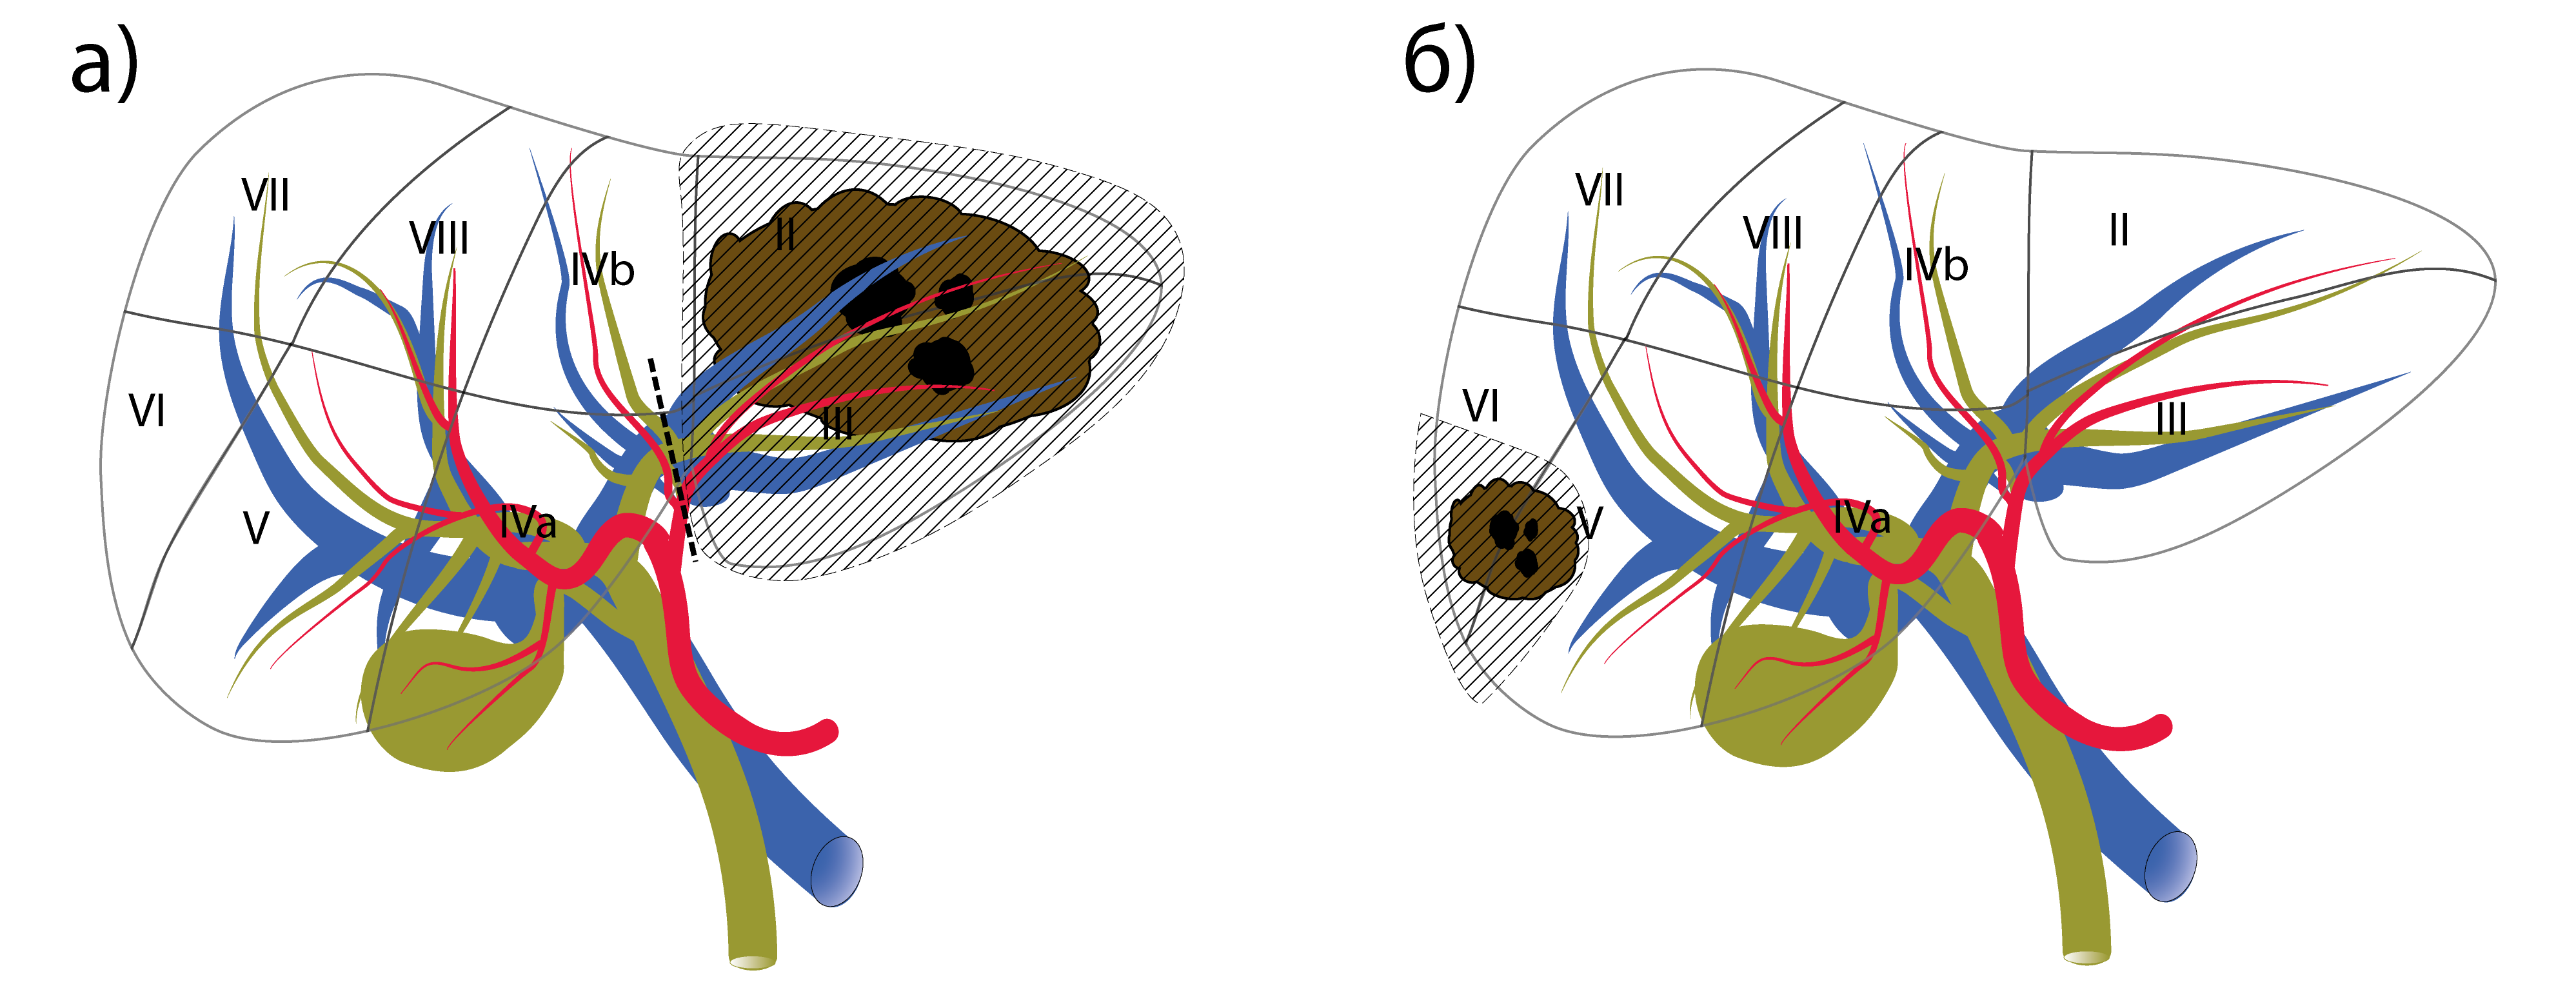
\includegraphics[width=\linewidth]{Figures/Anatomical vs marginal_Horizontal.png}
%  \checkparity This is an \pageparity\ page.%
  \caption{Прилади анатомічної (а) та крайової (б) резекції. При анатомічній резекції спочатку виділяють та пересікають судини, що живлять відповідні сегменти, а потім по лінії знекровлення проводять відсіченя паренїми. При крайовій енуклеорезекції лінія транссекції намічається з відступом 1-2 см від краю пухлини}
  \label{fig:textfig}
  %\zsavepos{pos:textfig}
\end{figure}

\newpage
\section{Як виконується відкрита (традиційна) резекція печінки?}

При відкритій або традиційній резекції печінки доступ до органа відбувається шляхом лапаротомії - великого розрізу на передній черевній стінці із наступним широким розведенням країв рани, що забезпечує хірургу максимально широке поле дії для операції. Такий доступ дозволяє виконувати надскладні операції при вростанні пухлин в великі судини печінки або жовчні протоки. 

\begin{marginfigure}[10pt]%
  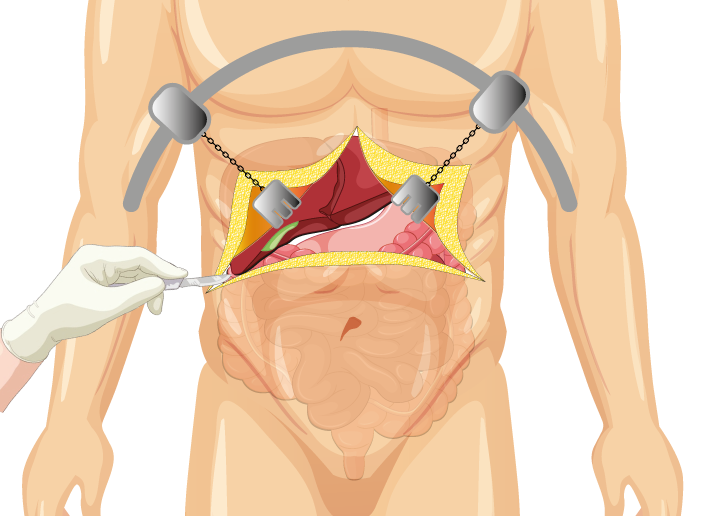
\includegraphics[width=\linewidth]{Figures/LapVsOpen_Open surgery.png}
  \caption{Схема хірургічного доступу при відкритій резекції печінки. Хірург оперує через широкий Т-подібний доступ типу "мерседес". Края рани розтягуються спеціальними ретракторами на лебідках.}
  \label{fig:crlm}
\end{marginfigure}

\section{Що таке лапароскопія?}

Лапароскопія  - це високотехнологічна хірургічна методика, яка дозволяє отримати зображення внутрішніх органів та проводити маніпуляції на них без розрізу передньої черевної стінки за рахунок спеціального ендовідеохірургічного обладнання.

Лапароскопічні операції - безпечний метод лікування, що застосовується у всіх сучасних клініках. На теперішньому етапі розвитку хірургії в лапароскопічному варіанті доступна абсолютна більшість хірургічних операцій. 

Через свої переваги для пацієнтів при певних видах операцій (наприклад холецистектомія - видалення жовчного міхура) лапароскопія стала золотим стандартом лікування, залишивши відкритий доступ лише для виключних випадків. 

Під час проведення лапароскопічної операції хірург маніпулює в черевній порожнині спеціальними довгими інструментами під контролем зображення з відеокамери, яке виводиться на високоякісний медичний монітор.\sidenote[][-120pt]{Зображення органів черевної порожнини потрапляє в відеокамеру через лапароскоп - хірургічний інструмент, який має форму довгої та тонкої металевої трубки, в середині якої знаходяться оптичні лінзи та оптоволокно. Технічно лапароскоп є медичним аналогом об’єктиву звичайної камери.

Лапароскоп та хірургічні інструменти в живіт пацієнта вводять через спеціальні порти - пристрої  у вигляді короткої трубки з клапаном, що дозволяють утримувати в  черевній порожнині вуглекислий газ, що створює робочий простір для хірурга. 
}


\begin{marginfigure}[40pt]%
  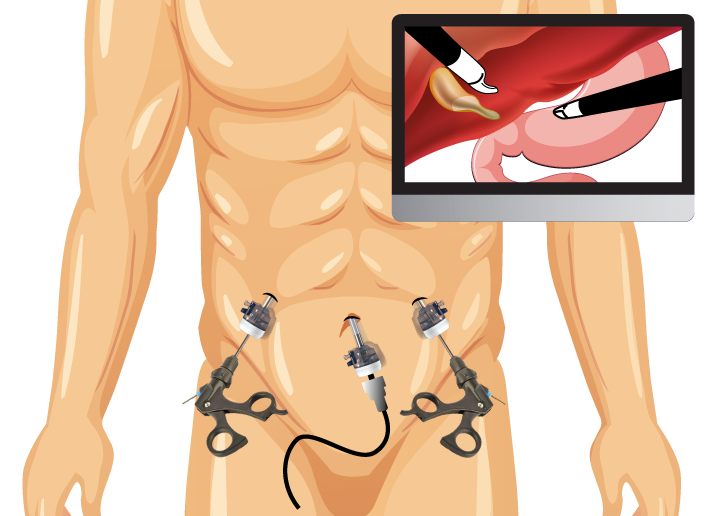
\includegraphics[width=\linewidth]{Figures/LapVsOpen_Laparoscopic surgery.png}
  \caption{Схема хірургічного доступу при лапароскопічній резекції печінки. Хірург оперує через маленькі розрізи спеціальними інструментами під контролем зображення, отриманого з відеокамери на моніторі}
  \label{fig:crlm}
\end{marginfigure}




\section{Що таке лапароскопічна резекція печінки?}

Лапароскопічна резекція печінки - це високотехнологічна хірургічна операція по видаленню частини печінки, яка виконується лапароскопічним шляхом, через маленькі проколи в черевній стінці під контролем відеокамери. 

\begin{tcolorbox}[width=\textwidth,colback=yellow!5!white,colframe=yellow!75!black]    
За об’ємом видаляємої паренхіми лапароскопічні резекції аналогічні відкритим, тобто для мініінвазивного підходу доступні всі ті самі об’єми операцій, включаючи обширні резекції, що і для традиційного.
\end{tcolorbox}    

Єдиним умовним обмеженням є вростання пухлини в магістральні судини або жовчні протоки.

Видалена частина печінки при лапароскопічних резекціях видаляється через невеликий атравматичний розріз, довжиною 5 см внизу живота.


\section{Які переваги надає лапароскопічна резекція печінки?}


Лапароскопічна резекція в порівнянні із відкритими операціями дозволяє хворому отримати:
\begin{itemize}
    \item аналогічний відкритим операціям онкологічний ефект при злоякісних захворюваннях
    \item меншу кількість післяопераційних ускладнень
    \item менш виражений больовий синдром та післяопераційний стрес
    \item пришвидшену реабілітацію та більш повне функціональне відновлення
    \item відсутність травматизації передньої черевної стінки та збереження функції м’язів преса
    \item кращий косметичний ефект
\end{itemize}
	

\section{Кому показана відкрита, а кому лапароскопічна резекція печінки?}

\begin{tcolorbox}[width=\textwidth,colback=green!5!white,colframe=green!75!black]    
В більшості випадків, при неускладнених формах пухлин будь-якого походження можливо виконати резекцію печінки в лапароскопічному варіанті, що надає пацієнту покращений профіль безпеки та адекватну онкологічну ефективність.
\end{tcolorbox}    

У випадку проростання пухлин в магістральні судини або жовчні протоки методом вибору залишається відкрита резекція печінки.

\section{Хто обирає об'єм резекції та хірургічний доступ?}
В процесі обстеження пацієнта хірург визначає покази до хірургічного лікування та його об'єм. Після отримання результатів обстеження хірург обговорює їх з пацієнтом, знайомить його з можливим планом лікування. За відсутності протипоказів під час цього обговорення пацієнт може віддати перевагу відкритому чи лапароскопічному варіанту виконання операції.
